
%-------------------------------------------------------------------------------
%							FOURTH SECTION
%-------------------------------------------------------------------------------


\section{\textsc{Travaux et résultats 2D}}


\subsection{Déplacement des n\oe{}uds}


\begin{frame}{Déplacement des n\oe{}uds d'un floe isolé (1)}

    \mycols{

        \mycol{40}{

            \begin{figure}
                \centering
                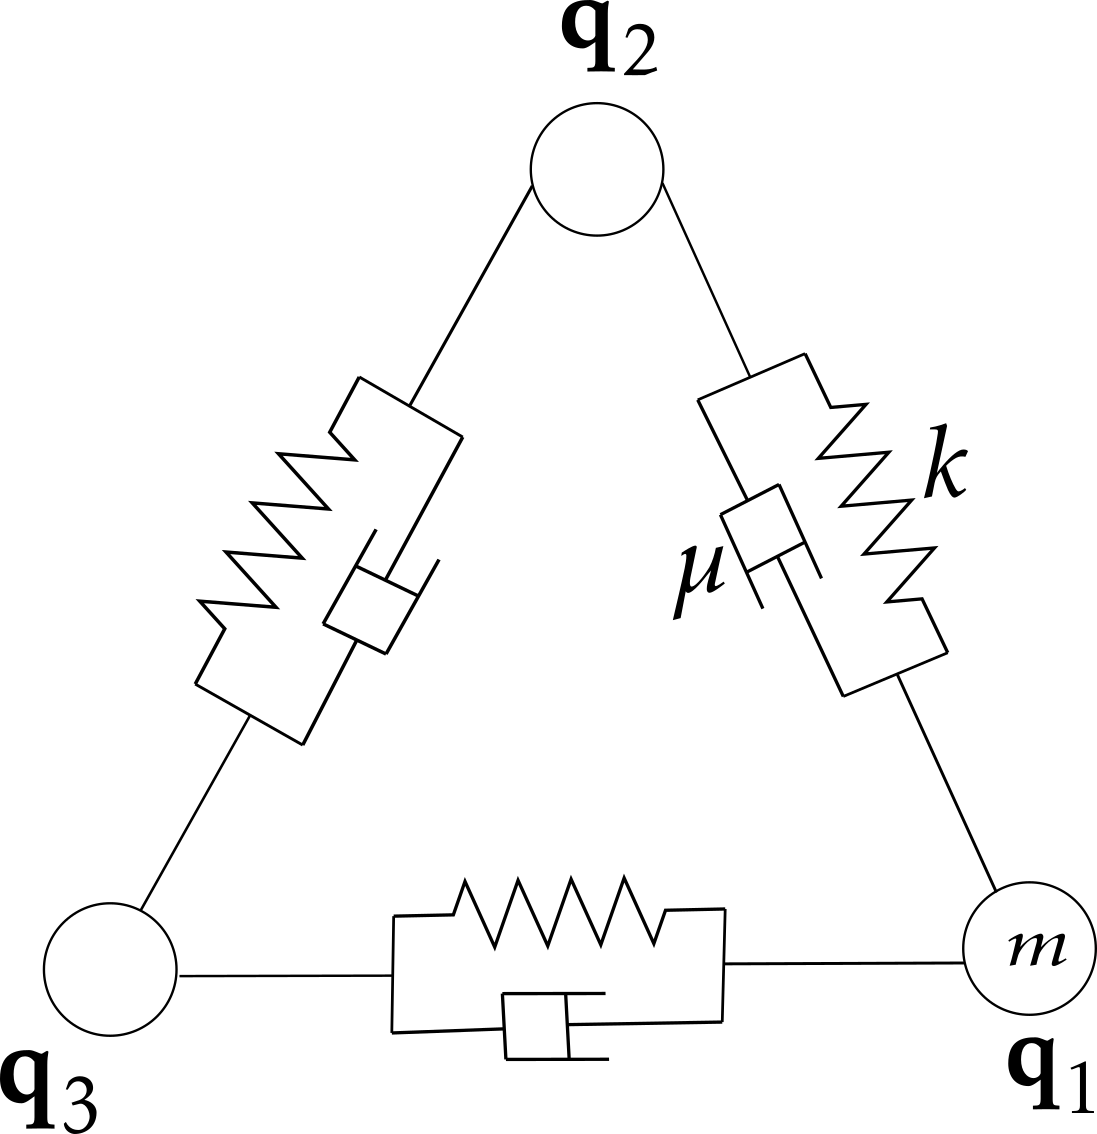
\includegraphics[width=0.6\textwidth]{Deplacement2D-1.png}
                \caption{Floe de glace 2D}
            \end{figure}

        }

        \mycol{60}{
            \myfig{PlotDeplacement2D-1-NonConv.png}{Simulation avec $T=10$}

            % \myfig{PositionInitFinales.png}{Illustration à $T=4$}
        }

    }

	\vspace{-0.5cm}
    Les équations de Newton-Euler :
    \begin{align*}
        \forall i \in \mathbb{Z}/3\mathbb{Z}, \quad m \ddot{\bvec{q}}_i = \underbrace{\sum_{j=i+1}^{i+2} \textcolor{teal}{C_{ij}} \left[  \textcolor{blue}{k \left( \Vert \bvec{q}_j - \bvec{q}_i \Vert - L_{ij} \right) \bvec{u}_{ij}} \textcolor{orange}{- \mu \left\langle \dot{\bvec{q}}_j - \dot{\bvec{q}}_i, \, \bvec{u}_{ij}  \right\rangle  \bvec{u}_{ij}}  \right]}_{\bvec F_i} . 
    \end{align*}

    Schéma d’Euler explicite :
    \begin{align*} \label{eq:systeme2D}
        \bvec{q}_{i}^{n+1} = 2\bvec{q}_{i}^{n}-\bvec{q}_{i}^{n-1} + \frac{\Delta t^2}{m} \sum_{j=i+1}^{i+2}C_{ij}\left[ k \left( \Vert \bvec{q}_j^n - \bvec{q}_i^n \Vert - L_{ij} \right) \bvec{u}_{ij} - \frac{\mu}{\Delta t} \left\langle \bvec{q}_{j}^{n}-\bvec{q}_{j}^{n-1} - \bvec{q}_{i}^{n}+\bvec{q}_{i}^{n-1}, \, \bvec{u}_{ij} \right\rangle  \bvec{u}_{ij}  \right].
    \end{align*}
    
\end{frame}


\begin{frame}[fragile]{Déplacement des n\oe{}uds d'un floe isolé (2)}

    \tiny
    \begin{lstlisting}[language=Python,caption=Code de simulation et schéma avec Scipy]
                                    q0 = np.stack([q1_0, dotq1_0, q2_0, dotq2_0, q3_0, dotq3_0])
                                    q0_ = np.reshape(q0, (nb_nodes*4))

                                    def model(t, Q_):
                                        Q = np.reshape(Q_, (nb_nodes*2, 2))
                                        Q_ret = np.zeros_like(Q)
                                        Q_ret[2*0] = 0; Q_ret[2*1] = 0
                                        
                                        for i in range(1, nb_nodes):  ## <-- Node 0 is immobilized
                                            Q_ret[2*i] = Q[2*i+1] 
                                            
                                            for neighbor in range(i+1, i+3):
                                                j = neighbor % nb_nodes
                                                u[i,j] = (Q[2*j] - Q[2*i]) / nplin.norm(Q[2*j] - Q[2*i])
                                                Q_ret[2*i+1] += (1 / m)*C[i,j]*( k*(nplin.norm(Q[2*j]-Q[2*i]) - L[i,j])*u[i,j]
                                                                -  mu*(np.dot(Q[2*j+1] - Q[2*i+1], u[i,j]))*u[i,j] )
                                        return np.reshape(Q_ret, (nb_nodes*4))

                                    sol = solve_ivp(model, [0,T], q0_, t_eval=t)
    \end{lstlisting}
    
	\hspace*{-1cm}
	\mycols{
	
	\mycol{70}{
	    \begin{figure}
        \centering
        \hspace{-1cm}
        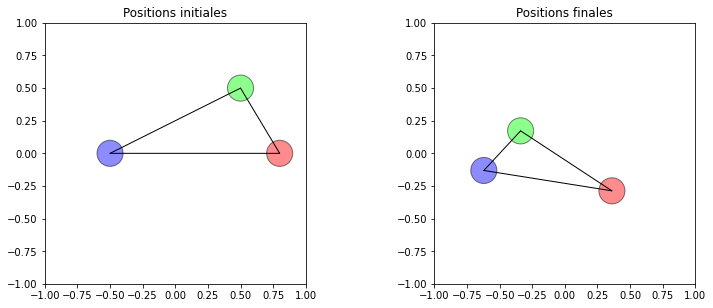
\includegraphics[width=0.8\textwidth]{PositionInitFinales.png}
        %\hspace{-1.5cm}
        \caption{Illustration à $t=0$ et $t=4$}
    	\end{figure}
	}
	
	\hspace{-0.5cm}
	
	
	\mycol{32}{
	\vspace{-0.5cm}
	\normalsize
	\hspace{-1cm}
	\begin{adjustwidth}{1cm}{2cm}
	   \begin{alertblock}{En somme}
         Avec un schéma Euler explicite, symplectique ou Scipy (RK45), il faut fixer certains n\oe{}uds pour que le système reste stable!
        \end{alertblock}
	\end{adjustwidth}	
	}	
	\normalsize
	}
	

\end{frame}




\subsection{Percussion entre floes}


\begin{frame}{Collision parfaitement inélastique entre deux floes (1)}

    \mycols{

        \mycol{40}{
			\myfigframe{Percussion2DNew.png}{Illustration de la percussion 2D}

\begin{align*}
\begin{dcases}
    (m+m') \ddot{\bvec{q}}_0  = \bvec{F}_0 + \bvec{F}^{'}_0  , & \textcolor{cyan}{\text{(SE)}} \\
    \ddot{\bvec{p}}_0 = \ddot{\bvec{q}}_0 , \dot{\bvec{p}}_0 = \dot{\bvec{q}}_0 , \bvec{p}_0 = \bvec{q}_0 - \Delta_0 , & \textcolor{cyan}{\text{(SE)}} \\
    m \ddot{\bvec{q}}_i = \bvec{F}_i   \,, \quad \quad \quad \forall 1 \leq i \leq n-1 , & \textcolor{orange}{\text{(SI)}} \\
    m' \ddot{\bvec{p}}_i = \bvec{F}^{'}_i   \,, \quad \quad \quad \forall 1 \leq i \leq n'-1 , & \textcolor{orange}{\text{(SI)}}
\end{dcases}
\end{align*}
où : $\quad \Delta_0 = \bvec{q}_0(0) - \bvec{p}_0(0)$.
			
        }

        \mycol{60}{
            \myfigframesize{Percussion2DSlides}{Un maillage 2D par processus de Poisson}{80}
            
            \centering
    \textcolor{mygray}{\href{run:../../../../Share/ShortAnim2D.gif}{\textbf{Animation de la percussion 2D}}}

    %\begin{adjustwidth}{-6em}{-6em}
		\animategraphics[loop,controls,autoplay,width=\linewidth]{10}{Simu2D/ShortAnim2D-}{0}{70}
    %\end{adjustwidth}	
	
        }

    }
    
\end{frame}




\begin{frame}{Collision parfaitement inélastique entre deux floes (2)}

	\myfigframesize{ClientWebMoi.jpg}{Client web développé et maintenu avec Flask}{60}
	\note{En fin je dois vous montrer ce clien web.  Je ne pouvais m'en empécher.}
    
\end{frame}
